\documentclass[border=10pt]{standalone}
\usepackage{tikz}

\begin{document}

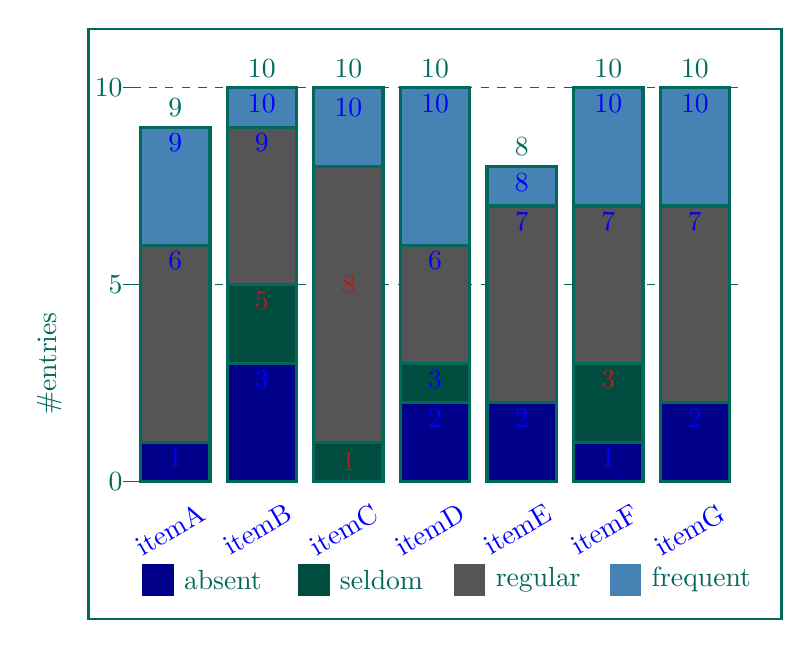
\begin{tikzpicture}[
    x=1.1cm, y=0.5cm
  ]
  % Define colors
  \definecolor{myframecolor}{HTML}{00695C} % Dark Teal
  \definecolor{myblue}{HTML}{00008B}       % Dark Blue
  \definecolor{myteal}{HTML}{004D40}       % Darker Teal
  \definecolor{mygrey}{HTML}{555555}       % Dark Grey
  \definecolor{mylightblue}{HTML}{4682B4}  % Steel Blue
  \definecolor{myred}{HTML}{B71C1C}        % Dark Red

  % Draw frame and axes
  \draw[myframecolor, thick] (0, -3.5) rectangle (8, 11.5);

  % Y-axis ticks and labels
  \foreach \y in {0, 5, 10} {
    \draw[myframecolor] (0.4, \y) -- (0.6, \y) node[left=3pt, myframecolor] {\y};
  }
  \node[myframecolor, rotate=90, anchor=south] at (-0.2, 3) {\#entries};

  % Grid lines
  \draw[myframecolor, dashed] (0.5, 5) -- (7.5, 5);
  \draw[myframecolor, dashed] (0.5, 10) -- (7.5, 10);

  % Data for the bars
  % Format: \x / label / absent / seldom / regular / frequent / total
  \foreach \x / \label / \dAbs / \dSel / \dReg / \dFreq / \tot in
    {1/itemA/1/0/5/3/9, 2/itemB/3/2/4/1/10, 3/itemC/0/1/7/2/10, 4/itemD/2/1/3/4/10, 5/itemE/2/0/5/1/8, 6/itemF/1/2/4/3/10, 7/itemG/2/0/5/3/10}
  {
    % X-axis label
    \node[blue, rotate=30, anchor=north east] at (\x+0.3, -0.2) {\label};
    % Total label
    \node[myframecolor] at (\x, \tot+0.5) {\tot};

    \pgfmathsetmacro{\barleft}{\x-0.4}
    \pgfmathsetmacro{\barright}{\x+0.4}
    
    % Special case for itemC due to anomalous labeling
    \ifnum\x=3
      \node[blue] at (3, 0.2) {0};
      \draw[fill=myteal, draw=myframecolor, line width=1.2pt] (\barleft, 0) rectangle (\barright, 1);
      \node[myred] at (3, 0.5) {1};
      \draw[fill=mygrey, draw=myframecolor, line width=1.2pt] (\barleft, 1) rectangle (\barright, 8);
      \node[myred] at (3, 5) {8};
      \draw[fill=mylightblue, draw=myframecolor, line width=1.2pt] (\barleft, 8) rectangle (\barright, 10);
      \node[blue] at (3, 9.5) {10};
    \else % General case for other items
      \pgfmathsetmacro{\y}{0}

      % Absent segment
      \ifdim\dAbs pt > 0pt
        \pgfmathsetmacro{\ynew}{\y+\dAbs}
        \draw[fill=myblue, draw=myframecolor, line width=1.2pt] (\barleft, \y) rectangle (\barright, \ynew);
        \pgfmathtruncatemacro{\labelval}{\ynew}
        \node[blue] at (\x, \ynew-0.4) {\labelval};
        \pgfmathsetmacro{\y}{\ynew}
      \fi

      % Seldom segment
      \ifdim\dSel pt > 0pt
        \pgfmathsetmacro{\ynew}{\y+\dSel}
        \draw[fill=myteal, draw=myframecolor, line width=1.2pt] (\barleft, \y) rectangle (\barright, \ynew);
        \pgfmathtruncatemacro{\labelval}{\ynew}
        \ifnum\x=2 \node[myred] at (\x, \ynew-0.4) {\labelval};
        \else\ifnum\x=6 \node[myred] at (\x, \ynew-0.4) {\labelval};
        \else \node[blue] at (\x, \ynew-0.4) {\labelval};
        \fi\fi
        \pgfmathsetmacro{\y}{\ynew}
      \fi

      % Regular segment
      \ifdim\dReg pt > 0pt
        \pgfmathsetmacro{\ynew}{\y+\dReg}
        \draw[fill=mygrey, draw=myframecolor, line width=1.2pt] (\barleft, \y) rectangle (\barright, \ynew);
        \pgfmathtruncatemacro{\labelval}{\ynew}
        \node[blue] at (\x, \ynew-0.4) {\labelval};
        \pgfmathsetmacro{\y}{\ynew}
      \fi

      % Frequent segment
      \ifdim\dFreq pt > 0pt
        \pgfmathsetmacro{\ynew}{\y+\dFreq}
        \draw[fill=mylightblue, draw=myframecolor, line width=1.2pt] (\barleft, \y) rectangle (\barright, \ynew);
        \pgfmathtruncatemacro{\labelval}{\ynew}
        \node[blue] at (\x, \ynew-0.4) {\labelval};
        \pgfmathsetmacro{\y}{\ynew}
      \fi
    \fi
  }

  % Legend
  \begin{scope}[shift={(0.8,-2.5)}]
    \node[fill=myblue, minimum size=4mm, inner sep=0pt, label={[myframecolor]right:absent}] at (0,0) {};
    \node[fill=myteal, minimum size=4mm, inner sep=0pt, label={[myframecolor]right:seldom}] at (1.8,0) {};
    \node[fill=mygrey, minimum size=4mm, inner sep=0pt, label={[myframecolor]right:regular}] at (3.6,0) {};
    \node[fill=mylightblue, minimum size=4mm, inner sep=0pt, label={[myframecolor]right:frequent}] at (5.4,0) {};
  \end{scope}

\end{tikzpicture}

\end{document}
